%% CoopGCN --- Array (Elsevier) submission
%% Layout: Elsevier CAS double-column class (cas-dc.cls), the class used by
%% the journal's published articles (cf. Array 30 (2026) 100986).
%% Structure follows specs/CoopGCN_Paper_Structure.md section by section.
%% Compile:  pdflatex coopgcn_array -> bibtex coopgcn_array -> pdflatex x2
%% Requires cas-dc.cls, cas-common.sty, cas-model2-names.bst (see ./cas/).
\documentclass[a4paper,fleqn,longmktitle]{cas-dc}

\usepackage[numbers]{natbib}
\usepackage{amsmath,amssymb}
\usepackage{algorithm}
\usepackage{algpseudocode}
\usepackage{tikz}
\usetikzlibrary{arrows.meta,positioning,calc,fit,backgrounds}

\newtheorem{proposition}{Proposition}
\newtheorem{definition}{Definition}
\newtheorem{corollary}{Corollary}

%% ---- black-only TikZ styles (monochrome, print-safe) --------------------
\tikzset{
  blk/.style   = {draw=black, line width=0.5pt, rectangle, align=center,
                  inner sep=3pt, font=\scriptsize},
  chan/.style  = {draw=black, line width=0.7pt, rectangle, align=left,
                  inner sep=4pt, font=\scriptsize, minimum width=4.05cm},
  band/.style  = {draw=black, line width=0.5pt, dashed, rectangle,
                  align=center, inner sep=4pt, font=\scriptsize},
  hdr/.style   = {font=\scriptsize\bfseries},
  ar/.style    = {-{Latex[length=1.6mm,width=1.2mm]}, line width=0.5pt},
  dar/.style   = {-{Latex[length=1.6mm,width=1.2mm]}, line width=0.5pt, dashed},
}

\begin{document}

\let\WriteBookmarks\relax
\def\floatpagepagefraction{1}
\def\textpagefraction{.001}

\shorttitle{Shapley-derived credit assignment in graph convolutional networks}
\shortauthors{M. Louhichi et al.}

\title[mode = title]{CoopGCN: Shapley-derived credit assignment in graph
convolutional networks via cooperative game theory for long-tail
recommendation}

\author[1]{Mouad Louhichi}[orcid=0000-0000-0000-0000]
\cormark[1]
\ead{mouad_louhichi@um5.ac.ma}
\credit{Conceptualization, Methodology, Software, Formal analysis,
Investigation, Data curation, Writing -- original draft, Visualization}

\author[1]{Redwane Nesmaoui}
\credit{Methodology, Validation, Formal analysis, Writing -- review and editing}

\author[1]{Mohamed Lazaar}
\credit{Conceptualization, Supervision, Project administration,
Writing -- review and editing}

\affiliation[1]{organization={National Higher School of Computer Science and
    Systems Analysis (ENSIAS), Mohammed V University in Rabat},
    city={Rabat},
    country={Morocco}}

\cortext[1]{Corresponding author.}

\begin{abstract}
Linear graph collaborative-filtering models weight interactions primarily by
topology and therefore provide no explicit account of which historical edges
contributed to a recommendation. We introduce \textbf{CoopGCN}, a
Shapley-derived architecture with three cooperative games: edge-level credit
($\mathbf{G_1}$), hyperedge-level group credit ($\mathbf{G_2}$), and
training-interaction valuation and pruning ($\mathbf{G_3}$). An SVD
contrastive channel supplies a global view, while a stop-gradient consistency
loss distils Monte-Carlo credit estimates into an attention network so that no
Shapley sampling is required at serving time.

We separate properties of the exact Shapley allocation from those of the
deployed model. Efficiency, symmetry, dummy player and additivity apply to the
allocation $\phi$; the sigmoid modulation preserves only within-degree credit
ordering, and attention distillation introduces an unbounded approximation gap.
A per-edge result bounds Channel-A weight deviation from its zero-credit
reference by $\lambda\epsilon/(4\tau\sqrt{d_ud_i})$; it is not a bound on
end-to-end ranking robustness.

Single-run measurements across five datasets and ten models provide
preliminary evidence of an accuracy--exposure trade-off. Among direct
hypergraph/cooperative peers, CoopGCN has the highest NDCG@20 on four of five
datasets and the highest Tail Recall and Coverage@20 on all five. On ML-1M,
however, it records NDCG@20 $=0.1994$, below all six graph comparators shown,
while attaining TR@20 $=0.0075$ and Coverage@20 $=40.7\%$. On Yelp2018 and
Amazon-Book it records the highest graph-model NDCG@20, 0.0376 and 0.0235.
GAT-CF is stronger on the two dense benchmarks but collapses on the three sparse benchmarks;
because its collapse is not yet supported by tuning traces, this comparison is
preliminary rather than a definitive verdict on attention. No multi-seed,
measured noise-injection, component-ablation, attribution-faithfulness, or
wall-clock study is available. We therefore claim evidence for a
regime-dependent distributional effect, not universal accuracy, robustness,
explainability, or efficiency superiority.
\end{abstract}

\begin{highlights}
\item Three cooperative games assign credit to edges, hyperedges and training
interactions in graph collaborative filtering.
\item Theoretical guarantees are restricted to Shapley credit; deployed
weights preserve only within-degree ordering up to distillation error.
\item Single-run measurements show strong tail exposure but an accuracy cost
on dense ML-1M.
\item CoopGCN leads direct hypergraph/cooperative peers in NDCG on four of five
measured datasets and in Tail Recall and Coverage on all five.
\item Serving performs no Monte-Carlo Shapley sampling; residual attention
latency remains unmeasured.
\end{highlights}

\begin{keywords}
Recommender systems \sep Graph convolutional networks \sep Cooperative game
theory \sep Shapley value \sep Popularity bias \sep Long-tail recommendation
\sep Robustness to noisy interactions \sep Credit assignment
\end{keywords}

\maketitle

%==========================================================================
\section{Introduction}
\label{sec:intro}

Single-run measurements on MovieLens-1M reveal a sharp accuracy--exposure
trade-off. CoopGCN records lower NDCG@20 than the six graph comparators in our
measured table, yet it is the only hypergraph/cooperative model with non-zero
Tail Recall at cut-off 20 and exposes 40.7\% of the catalogue rather than the
8--10\% reached by its direct peers. On sparse Yelp2018 and Amazon-Book it
also records the highest NDCG@20 among the measured graph models. These
observations motivate, but do not statistically establish, the hypothesis
that interaction-level credit matters most in sparse, high-cardinality
settings.

Graph recommenders' narrow catalogue exposure, sensitivity to noisy data and
lack of per-interaction attribution are often treated as separate problems.
We investigate whether they share a design limitation inherited from
LightGCN: propagation has no explicit representation of how much a particular
interaction contributes. Noise resilience and attribution faithfulness are
mechanistic hypotheses in this manuscript, not measured findings. Throughout,
\emph{credit assignment} means allocating training and propagation influence;
it does not mean that the credits are faithful human-facing explanations. We
treat explanation faithfulness as a separate, unexecuted evaluation protocol
in Section~\ref{sec:xai-protocol}.

\subsection{The LightGCN paradigm and its core trade-off}
\label{sec:paradigm}

Graph convolutional networks reshaped collaborative filtering (CF) by
modelling user--item interaction histories as bipartite graphs. NGCF
\citep{wang2019ngcf} demonstrated the value of high-order connectivity, and
LightGCN \citep{he2020lightgcn} then showed that the feature-transformation
matrices and nonlinear activations inherited from generic GCNs cause
oversmoothing and training instability in pure CF. Removing them reduces
message passing to symmetric-normalised linear aggregation,
\begin{equation}
\mathbf{E}^{(k+1)} = \left( \mathbf{D}^{-\frac{1}{2}} \mathbf{A}
\mathbf{D}^{-\frac{1}{2}} \right) \mathbf{E}^{(k)},
\label{eq:lightgcn}
\end{equation}
which with mean layer pooling and a Bayesian Personalized Ranking objective
\citep{rendle2009bpr} established an empirical floor that has proved
remarkably hard to beat.

The three equations defining LightGCN encode three silent assumptions: every
neighbour is aggregated with weight $1/\sqrt{d_u d_i}$, every layer is pooled
equally, and every negative is sampled uniformly. The first is our concern
here. It fixes the influence of neighbour $i$ on user $u$ at a quantity
determined \emph{entirely by graph topology}, with no dependence on what the
interaction meant.

Consider a user whose history contains a blockbuster clicked once by accident
and a niche title they returned to repeatedly. Equation~\eqref{eq:lightgcn}
weights these by degree alone. Worse, because the coefficient is
degree-normalised and the blockbuster has the larger degree, the accidental
click is down-weighted for a reason that has nothing to do with its being
accidental---and the niche title is up-weighted for a reason that has nothing
to do with its being meaningful. The ordering happens to be right; the
mechanism producing it is blind. Where degree and informativeness diverge, as
they do for popular-but-incidental and rare-but-deliberate interactions alike,
the model has no parameter with which to tell them apart.

Three consequences follow directly, and they are precisely the three symptoms
above. The model cannot \emph{denoise}, because it cannot identify a
low-value edge. It cannot \emph{explain}, because it has no per-interaction
attribution to report. And it cannot \emph{resist} an adversary, because an
injected edge is trusted exactly as much as an observed one.

\subsection{Four structural failure modes of unweighted propagation}
\label{sec:failuremodes}

A systematic analysis reveals that LightGCN's remaining weaknesses are
precisely the capabilities its simplification discarded. We label them
$\mathbf{W_k}$ here and expand the labelling into a full twelve-category
taxonomy in Section~\ref{sec:taxonomy}.

\begin{enumerate}
\item \textbf{Flat credit and uniform neighbour weighting
($\mathbf{W_1}, \mathbf{W_2}$).} Every neighbour contributes with an immutable
topological weight. Because that weight is degree-normalised, noisy or
irrelevant edges dilute the embedding quality of every node they touch, and
the model has no parameter with which to discount them.

\item \textbf{Pairwise-only topological bias ($\mathbf{W_5}$).} Bipartite
edges capture relations $(u,i)$ but cannot represent higher-order group units
such as shopping sessions, item categories or multi-item bundles, which must
instead be approximated by cliques.

\item \textbf{Popularity-bias amplification and dimensional collapse
($\mathbf{W_3}, \mathbf{W_8}$).} Repeated convolution is dominated by the
leading eigenvectors of the adjacency matrix. Embeddings collapse toward
high-degree items, and tail recall degrades sharply with layer depth.

\item \textbf{Vulnerability to noisy and poisoned data ($\mathbf{W_{10}}$).}
Because every edge is trusted uniformly, malicious clicks or erroneous
interactions ripple unconstrained through $k$-hop neighbourhoods.
\end{enumerate}

Section~\ref{sec:taxonomy} expands these into a twelve-category taxonomy and
argues that the high-severity entries reduce to three root causes.

\subsection{The game-theoretic perspective}
\label{sec:perspective}

The natural response is to make the weights learnable, and graph attention
does exactly that. Our position is that this is the right instinct applied
with the wrong tool, and the reason is worth stating precisely.

Predicting a preference score $s_{ui} = \bar{\mathbf{e}}_u \cdot
\bar{\mathbf{e}}_i$ is a problem of \emph{team production}: the pooled
embedding $\bar{\mathbf{e}}_u$ is generated jointly by the neighbours in
$\mathcal{N}(u)$, and no single neighbour produces it alone. Asking how much
each contributed is not merely analogous to a cooperative game---it is one,
namely $\Gamma_u = (\mathcal{N}(u), v_u)$, with the neighbours as players and
representation quality as the characteristic function.

This matters because cooperative game theory answers the question
\emph{uniquely}. The Shapley value \citep{shapley1953value} is the only
allocation satisfying efficiency (all credit is distributed), symmetry
(equal contributions earn equal credit), dummy player (a null contributor
earns zero), and additivity (credit decomposes linearly across objectives).
Attention weights satisfy none of the four, and two of the failures are
consequential rather than cosmetic.

\emph{Symmetry} forbids assigning different Shapley credit when marginal
utilities are equal. This is exactly the channel through which popularity bias
enters Eq.~\eqref{eq:lightgcn}, and nothing in an attention module's objective
closes it: if degree-correlated weights lower training loss---which on
head-heavy data they typically do---attention will learn them. The Shapley allocation cannot do so: symmetry constrains credit rather than
expressing a preference in a loss. The deployed propagation coefficient still
contains degree normalisation, so this statement does not imply degree-invariant
full weights.

\emph{Dummy player} assigns exactly zero credit to a neighbour whose marginal
contribution vanishes in every coalition. A maliciously injected edge is close
to such a player only when its marginal utility is uniformly small; random or
targeted injection does not guarantee that condition.

We must immediately qualify what this buys, because the distinction governs
every theoretical claim in this paper. The axioms characterise the
\emph{allocation} $\phi$. They do not automatically characterise the
propagation weight we deploy, which is a bounded, strictly positive transform
of $\phi$ (Eq.~\eqref{eq:edgeweight}). A dummy player receives $\phi = 0$ and
therefore the \emph{minimum} attainable modulation, not zero weight. What the
axioms deliver is a principled, monotone ordering of neighbours by contribution
together with a floor on how little influence a worthless edge can retain;
what they do not deliver is deletion of that edge. We therefore describe
CoopGCN throughout as \emph{Shapley-derived} rather than axiom-preserving at
the deployed-weight level,
and Section~\ref{sec:gap} makes the separation precise.

The distinction between axiomatic and heuristic credit is therefore an
empirical question with a sharp form---\emph{is Shapley just expensive
attention?}---which we formalise in Section~\ref{sec:central} as a
make-or-break ablation with a victory condition fixed in advance.

\subsection{Summary of contributions}
\label{sec:contrib}

\begin{enumerate}
\item \textbf{A diagnosis, not a list.} We catalogue twelve representational
and training weaknesses of linear graph CF, grade them by severity, map each
to the literature documenting it, and show that the high-severity subset
reduces to three root causes---credit is flat, structure is pairwise-only, and
the training recipe amplifies the head (Section~\ref{sec:taxonomy}). Each
recent improvement to LightGCN patches exactly one; CoopGCN targets all three.

\item \textbf{Tri-level cooperative game framework.} We formulate cooperative
games at the edge level ($\mathbf{G_1}$), hyperedge level ($\mathbf{G_2}$,
extending DyHuCoG) and data level ($\mathbf{G_3}$, TMC-Shapley valuation on
holdout NDCG), giving explicit characteristic functions for each and combining
them in a single trainable architecture (Section~\ref{sec:arch}).

\item \textbf{Theory that constrains the design.} We prove that Channel~A
recovers LightGCN propagation at $\lambda = 0$ when all other channels are
disabled, and reduces to a scalar-modulated family under symmetric utility
(Proposition~\ref{prop:recovery}). For a single Channel-A edge, deviation from
the zero-credit reference is at most
$\lambda\epsilon/(4\tau\sqrt{d_ud_i})$
(Proposition~\ref{prop:robust}). Section~\ref{sec:gap} explains why neither
statement is a guarantee about the complete deployed model or ranking
robustness.

\item \textbf{Shapley-derived credit distilled out of the serving path.} A
stop-gradient EMA consistency loss trains learnable attention to track Shapley
credits, so all Monte-Carlo computation is confined to training
(Section~\ref{sec:zero}). We report this as an architectural property; the
wall-clock cost of the residual attention network is not measured
(Section~\ref{sec:limitations}).

\item \textbf{Leakage-audited preliminary measurement with explicit
limits.} A common temporal protocol provides single-run measurements for ten
models on five datasets. The data support a distributional advantage and
sparse-regime competitiveness, but not universal accuracy superiority.
Projection-only ablations and noise curves have been removed from the evidence
section rather than presented as findings (Sections~\ref{sec:provenance} and
\ref{sec:limitations}).
\end{enumerate}

\paragraph{Objectives}
The \emph{primary objective} of this study is to determine whether Shapley-derived
credit assignment is a viable
replacement for the fixed degree-normalised weighting of linear graph CF---and
specifically whether it changes long-tail exposure without sacrificing
top-$K$ accuracy. Noise resilience and serving cost are pre-specified but
currently unmeasured secondary questions. The other objectives are: (i) to
establish that Channel~A contains LightGCN propagation as a boundary case; (ii)
to specify an ablation capable of quantifying each game level, while reporting
that measured component effects are not yet available; (iii) to compare the
Shapley-derived route with heuristic learnable attention under
matched capacity---the central question of the paper, for which we fix a
victory condition in advance in Section~\ref{sec:central}; and (iv) to report
every number with explicit provenance so that the boundary between measured,
measured and unmeasured evidence is visible to the reader.

\paragraph{Roadmap}
Section~\ref{sec:related} surveys related work and presents the taxonomy;
Section~\ref{sec:theory} develops the axiomatic foundation and the two
propositions; Section~\ref{sec:arch} specifies the architecture;
Section~\ref{sec:complexity} analyses cost; Section~\ref{sec:design} details
the protocol; Section~\ref{sec:results} reports results against RQ1--RQ5; and
Section~\ref{sec:conclusion} concludes with limitations and future work.

%==========================================================================
\section{Related work and systematic taxonomy}
\label{sec:related}

\subsection{Graph convolutional networks in collaborative filtering}
\label{sec:rw-gcn}

Graph convolution for recommendation descends from spectral GCNs
\citep{kipf2017gcn}, whose symmetric-normalised propagation rule LightGCN
ultimately inherits. NGCF \citep{wang2019ngcf} introduced GCNs for
collaborative filtering; LightGCN \citep{he2020lightgcn} removed
nonlinearities and transformation matrices, yielding
Eq.~\eqref{eq:lightgcn}. Subsequent work has largely
addressed one weakness at a time. LightGCN++ \citep{lee2024lightgcnpp}
diagnosed embedding-norm inflexibility and uniform neighbour weighting,
proposing learnable scalar norm scaling and node-degree weighting; it is the
strongest coverage-oriented baseline in our study and, by
Proposition~\ref{prop:recovery}, a constrained case of the present framework.
UltraGCN \citep{mao2021ultragcn} discards explicit message passing in favour
of a limit objective, and GF-CF \citep{shen2021powerful} recasts CF as graph
filtering. Contrastive and denoising models form a parallel line: SGL
\citep{wu2021sgl} augments the graph by stochastic dropout under an InfoNCE
objective; SimGCL \citep{yu2022simgcl} shows uniform embedding-space noise
outperforms structural augmentation; XSimGCL \citep{yu2024xsimgcl} simplifies
this further to a single-pass noise perturbation and, importantly for us,
attributes its long-tail benefit to more uniformly distributed
representations rather than to any notion of interaction value; and LightGCL
\citep{cai2023lightgcl} replaces stochastic augmentation with SVD-truncated
contrastive augmentation. We adopt the LightGCL-style channel because its
determinism composes cleanly with Monte-Carlo Shapley estimation. A recent
survey of self-supervised recommendation \citep{yu2024sslsurvey} confirms the
pattern across this family. Critically, all of these methods retain
topology-determined, value-agnostic edge weights: contrastive learning changes
the \emph{distribution} of embeddings but never asks which edge earned its
influence.

Two further lines are directly relevant because they attack the same symptoms
by other means. \emph{Attention} was the first attempt to make neighbour
weights adaptive: GAT \citep{velickovic2018gat} assigns learned coefficients
via masked self-attention, and this is precisely the heuristic alternative
against which our axiomatic construction is positioned
(Section~\ref{sec:central}). \emph{Denoising} methods target edge reliability
directly---T-CE \citep{wang2021denoising} down-weights high-loss interactions
as likely false positives, and RGCF \citep{tian2022rgcf} combines hard pruning
with soft reliability weights inside GNN message passing. RGCF is the closest
prior work in spirit to our $\mathbf{G_1}$: both modulate propagation by an
estimated per-edge reliability. The difference is the source of that estimate.
RGCF learns reliability from training loss, which is a model-internal signal
that can rationalise its own errors; $\mathbf{G_1}$ derives it from marginal
contribution to a held-out value function, and inherits a dummy-player property at the credit level: a non-contributing
edge receives zero Shapley credit and therefore the minimum modulation, not
zero propagation weight.

Two methodological studies inform our evaluation design. Dacrema et al.
\citep{dacrema2019worrying} showed that many reported neural recommender gains
vanish against properly tuned baselines, motivating our symmetric tuning
budget; and replication analyses of LightGCN \citep{peska2023lightgcn}
document that reported numbers swing materially with normalisation and split
choices, motivating the leakage audit of Section~\ref{sec:leakage}.

\subsection{Hypergraph recommender systems}
\label{sec:rw-hyper}

DHCN \citep{xia2021dhcn} and HCCF \citep{xia2022hccf} demonstrated that
hypergraph convolutional channels capture session-level and category-level
group structures, and HPCF \citep{chen2024hpcf} added local--global projection.
DyHuCoG \citep{louhichi2026dyhucog} pioneered preference-aware Monte-Carlo
Shapley weighting for hypergraph recommenders, injecting coalition-derived
contribution scores as dynamic hyperedge weights.

Our work extends DyHuCoG in three respects, summarised in
Table~\ref{tab:vsdyhucog}: we introduce edge-level Shapley weighting
($\mathbf{G_1}$), integrate data valuation ($\mathbf{G_3}$), and add an SVD
contrastive channel to prevent dimensional collapse. In our framework DyHuCoG
is exactly the $\mathbf{G_2}$-only configuration, which is why it serves as the
direct ablation target throughout Section~\ref{sec:results}.

\begin{table}[t]
\centering
\caption{CoopGCN relative to DyHuCoG, its direct predecessor and the
$\mathbf{G_2}$-only configuration of the present framework.}
\label{tab:vsdyhucog}
\footnotesize
\begin{tabular}{p{1.35cm}p{2.35cm}p{3.05cm}}
\toprule
\textbf{Dimension} & \textbf{DyHuCoG} & \textbf{CoopGCN (this work)} \\
\midrule
Shapley scope & Hyperedge weighting ($\mathbf{G_2}$) only & Edges
($\mathbf{G_1}$) $+$ hyperedges ($\mathbf{G_2}$) $+$ data ($\mathbf{G_3}$) \\
Propagation & Hypergraph only & Dual channel: pairwise graph $+$ hypergraph \\
Dimensional collapse & Not addressed & SVD-truncated contrastive view \\
Inference path & Game computed at inference & No MC sampling via
$\mathcal{L}_{\mathrm{game}}$ \\
Protocol & Random splits & Temporal split $+$ leakage audit \\
\bottomrule
\end{tabular}
\end{table}

\subsection{Explainable AI and Shapley values in machine learning}
\label{sec:rw-xai}

Shapley \citep{shapley1953value} established the unique allocation satisfying
efficiency, symmetry, dummy and additivity. Lundberg and Lee
\citep{lundberg2017shap} unified feature attribution via SHAP; Ghorbani and
Zou \citep{ghorbani2019datashapley} introduced Data Shapley for training-set
valuation; and prior work by the present authors applied Shapley values to
explaining unsupervised clustering and black-box models
\citep{louhichi2023shapley}. The obstacle to using Shapley values \emph{inside}
a model rather than as post-hoc explanation is cost: exact computation
requires $O(2^{|\mathcal{N}|})$ evaluations. Section~\ref{sec:complexity}
describes the restricted coalitions, permutation sampling and periodic refresh
that make in-training estimation tractable, and Section~\ref{sec:zero} removes
the cost from inference entirely.

\subsection{Explaining graph neural networks}
\label{sec:rw-gnnxai}

A parallel literature explains \emph{trained} GNNs post hoc. GNNExplainer
\citep{ying2019gnnexplainer} learns a soft edge/feature mask maximising mutual
information with the prediction; PGExplainer \citep{luo2020pgexplainer}
amortises that search into a parametric network so explanations generalise
inductively; and SubgraphX \citep{yuan2021subgraphx} searches connected
subgraphs by Monte-Carlo tree search scored with Shapley values. The taxonomic
survey of Yuan et al. \citep{yuan2023taxonomic} organises this space and, more
usefully for us, standardises the fidelity/sparsity metrics by which such
methods are judged --- the metrics our Section~\ref{sec:xai-protocol} adopts.

SubgraphX is the closest prior work in machinery, since it too computes
Shapley values over graph structure, and the distinction is worth stating
precisely because it is easy to miss. SubgraphX is \emph{post hoc and
explanatory}: the model is frozen, and Shapley values are computed afterwards
to describe a decision already made. CoopGCN is \emph{intrinsic and
constitutive}: Shapley values are computed during training and change the
propagation weights, so they alter the decision rather than describing it.
The two are complementary rather than competing --- one could run SubgraphX on
a trained CoopGCN. This also means the comparison is not head-to-head on
accuracy; the appropriate comparison, which we do not run, is whether
CoopGCN's intrinsic credits are as faithful as SubgraphX's post-hoc ones
(Section~\ref{sec:xai-protocol}).

The relationship to FastSHAP \citep{jethani2022fastshap} is closer still on
the mechanics: FastSHAP trains a network to emit Shapley values in a single
forward pass, which is precisely the amortisation our
$\mathcal{L}_{\mathrm{game}}$ performs for $a_{ui}$. We differ in purpose ---
FastSHAP amortises to accelerate explanation, we amortise to remove
game-theoretic computation from the serving path --- but the approximation
question their work raises applies directly to ours, and
Section~\ref{sec:gap} states it as the unbounded quantity $\delta$. Covert et
al. \citep{covert2021removing} give the unifying account of removal-based
explanation that clarifies which axioms survive which approximations, and we
follow their framing in separating properties of $\phi$ from properties of the
deployed weight.

\subsection{Popularity bias mitigation and robustness}
\label{sec:rw-bias}

Popularity bias in graph CF is well documented and systematised in the survey
of Chen et al. \citep{chen2023biassurvey}: convolution moves users toward
high-degree items, and tail exposure falls as depth grows
\citep{xia2022hccf,cai2023lightgcl}. Mitigations fall into four families,
distinguished by \emph{where in the pipeline} they intervene.
\emph{Re-ranking} post-processes the finished list, as in the personalised
xQuAD variant of Abdollahpouri et al. \citep{abdollahpouri2019managing}.
\emph{Regularisation} penalises popularity correlation inside the
learning-to-rank objective \citep{abdollahpouri2017controlling}.
\emph{Causal} methods model popularity as a confounder and remove its effect
by intervention: PDA \citep{zhang2021pda} deconfounds item popularity, while
DecRS \citep{wang2021decrs} intervenes on the user representation to curb bias
amplification. \emph{Representation-level} methods such as contrastive
augmentation act on the embedding distribution \citep{yu2024xsimgcl}.

CoopGCN belongs to none of the four, and the distinction is structural rather
than terminological. Re-ranking accepts a biased scorer and repairs its
output; regularisation and causal deconfounding correct the objective or the
inference rule while leaving the aggregation weights topological; contrastive
methods reshape the embedding geometry. CoopGCN instead changes the
\emph{aggregation coefficient itself}, so tail exposure is a consequence of
the weighting rule rather than a correction applied around it. The practical
difference is that no trade-off parameter has to be tuned to buy coverage back
after the fact.

On robustness, standard graph CF trusts all edges equally, an assumption
inherited from the confidence-weighted implicit-feedback formulation
\citep{hu2008wrmf} in which confidence is a function of frequency alone. The
threat model matters here: Z\"ugner et al. \citep{zugner2018adversarial} showed
that graph neural networks are vulnerable to \emph{targeted} structural
perturbations optimised against the model, which are strictly stronger than
the random edge injection protocol pre-specified in Section~\ref{sec:rq34}.
The retained measured record contains no random- or targeted-injection result,
so we make no empirical robustness claim. Data
Shapley \citep{ghorbani2019datashapley} established that valuing and pruning
low-contribution samples improves robustness, which $\mathbf{G_3}$ adapts to
the interaction graph. Whether contrastive augmentation or data valuation provides protection under
this protocol remains an open empirical question.

\subsection{Systematic taxonomy of limitations}
\label{sec:taxonomy}

Table~\ref{tab:weaknesses} catalogues twelve weaknesses of linearised graph
CF, separated into representational (W1--W6) and training/data (W7--W12)
categories. Reading it vertically rather than row by row, the high-severity
entries reduce to three root causes. \emph{Credit is flat} (W1, W2, W10): the
aggregation coefficient is identical for a decade-old rating and a purchase
made last night, and the model never asks how much a specific interaction
contributed---precisely a cooperative-game question. \emph{Structure is
pairwise-only} (W5, W9): preference lives in groups, and pairwise edges
approximate groups poorly exactly where data is sparse and group evidence is
strongest. \emph{The recipe amplifies the head} (W3, W7, W8): uniform
negatives, uniform weights and mean pooling jointly reward recommending
popular items. Each recent improvement to LightGCN patches exactly one of the
three; CoopGCN is organised to attack all three simultaneously.

\begin{table*}[t]
\centering
\caption{Systematic taxonomy of twelve weaknesses of linearised graph
collaborative filtering. Severity is our assessment of the magnitude of the
reported effect. The final column records how CoopGCN addresses each:
$\mathbf{G_1}$/$\mathbf{G_2}$/$\mathbf{G_3}$ denote the game level, C the
contrastive channel, R the training recipe, and P the evaluation protocol.}
\label{tab:weaknesses}
\small
\begin{tabular}{llp{6.5cm}lp{3.0cm}l}
\toprule
\textbf{\#} & \textbf{Weakness} & \textbf{Consequence} & \textbf{Severity} &
\textbf{Documented by} & \textbf{Addressed} \\
\midrule
\multicolumn{6}{l}{\textit{Representational weaknesses}} \\
\midrule
W1 & Uniform neighbour weighting & A misclick and a passion interaction
propagate identically; noisy neighbours dilute every node they touch & High &
LightGCN++ \citep{lee2024lightgcnpp} & $\mathbf{G_1}$ \\
W2 & Embedding-norm inflexibility & Norm carries no information yet cannot be
used; layer-0 and layer-$k$ norms are inconsistent, miscalibrating pooling &
High & LightGCN++ \citep{lee2024lightgcnpp} & $\mathbf{G_1}$, R \\
W3 & Dimensional collapse & Repeated propagation is dominated by leading
eigenvectors; the space becomes head-heavy & High & LightGCL
\citep{cai2023lightgcl} & C \\
W4 & Oversmoothing with depth & Performance peaks at 2--3 layers; deep
structure is unusable & Medium & LightGCN \citep{he2020lightgcn} & C \\
W5 & No beyond-pairwise structure & Sessions, categories and bundles must be
approximated by cliques & Medium & HCCF \citep{xia2022hccf} & $\mathbf{G_2}$ \\
W6 & Static, non-temporal embeddings & Recency and preference drift are
invisible & Medium & gSASRec \citep{petrov2023gsasrec} & --- (future work) \\
\midrule
\multicolumn{6}{l}{\textit{Training and data weaknesses}} \\
\midrule
W7 & BPR with one uniform negative & Under-samples hard negatives;
overconfidence inflates head-item scores & High & gSASRec
\citep{petrov2023gsasrec} & R \\
W8 & Popularity-bias amplification & Convolution moves users toward popular
items; tail recall falls as depth grows & High & HCCF \citep{xia2022hccf},
LightGCL \citep{cai2023lightgcl} & $\mathbf{G_1}$, $\mathbf{G_2}$, C \\
W9 & Cold start & New nodes have nothing to propagate & Medium & ---
& --- (future work) \\
W10 & No robustness to noisy or poisoned edges & One malicious interaction
ripples through $k$-hop neighbourhoods & Medium & Data Shapley
\citep{ghorbani2019datashapley} & $\mathbf{G_1}$, $\mathbf{G_3}$ \\
W11 & Evaluation leakage in the standard protocol & Reported numbers are
inflated; popularity baselines close much of the gap & High &
\citep{dacrema2019worrying} & P \\
W12 & Replication fragility & Results swing with normalisation, depth and
splits & Medium & \citep{peska2023lightgcn} & P \\
\bottomrule
\end{tabular}
\end{table*}

%==========================================================================
\section{Theoretical foundations: axiomatic credit assignment}
\label{sec:theory}

\subsection{Cooperative games and the Shapley value}
\label{sec:coopgame}

\begin{definition}[Cooperative game]
\label{def:game}
A cooperative game in characteristic function form is a pair $\Gamma =
(\mathcal{N}, v)$ where $\mathcal{N} = \{1,\dots,n\}$ is a finite set of
players---interaction neighbours, hyperedge members or training samples---and
$v : 2^{\mathcal{N}} \to \mathbb{R}$ is a characteristic value function with
$v(\emptyset) = 0$. The value $v(S)$ measures the utility achieved by coalition
$S \subseteq \mathcal{N}$.
\end{definition}

The Shapley value $\phi_i(\Gamma)$ assigns to player $i$ its average marginal
contribution across all permutation orderings:
\begin{equation}
\phi_i(\Gamma) = \!\!\sum_{S \subseteq \mathcal{N} \setminus \{i\}}\!\!
\frac{|S|!\,(|\mathcal{N}| - |S| - 1)!}{|\mathcal{N}|!}
\bigl[ v(S \cup \{i\}) - v(S) \bigr].
\label{eq:shapley}
\end{equation}
Table~\ref{tab:notation} fixes the notation used throughout.

\begin{table}[t]
\centering
\caption{Notation.}
\label{tab:notation}
\footnotesize
\begin{tabular}{ll}
\toprule
\textbf{Symbol} & \textbf{Definition} \\
\midrule
$\mathcal{G}=(\mathcal{U},\mathcal{I},\mathcal{E})$ & Bipartite graph, built
from the training split only \\
$\mathcal{N}(u)$ & Item neighbourhood of user $u$ (players in $\Gamma_u$) \\
$d_u, d_i$ & Node degrees in $\mathcal{G}$ \\
$\mathbf{e}^{(k)}_u,\mathbf{e}^{(k)}_i$ & Layer-$k$ embeddings,
$\in\mathbb{R}^{d}$ \\
$\bar{\mathbf{e}}_u,\bar{\mathbf{e}}_i$ & Pooled embeddings
$\sum_{k}\alpha_k\mathbf{e}^{(k)}$ \\
$s_{ui}$ & Preference score
$\bar{\mathbf{e}}_u \cdot \bar{\mathbf{e}}_i$ \\
$\mathcal{H}=(\mathcal{V},\mathcal{E}_H)$ & Hypergraph; $D_v,D_h$ degree
matrices \\
$\Gamma=(\mathcal{N},v)$ & Cooperative game with value function $v$ \\
$\phi_j,\hat{\phi}_j$ & Exact and Monte-Carlo Shapley value of player $j$ \\
$w_{ui}$ & Edge weight in Channel A ($\mathbf{G_1}$) \\
$\beta_h$ & Hyperedge weight in Channel B ($\mathbf{G_2}$) \\
$\gamma_{ui}$ & Sample weight from $\mathbf{G_3}$, $\in[1,1+\kappa]$ \\
$a_{ui}$ & Learnable attention logit distilled from
$\bar{\hat{\phi}}_{ui}$ \\
$\bar{\hat{\phi}}_{ui}$ & EMA of historical Shapley estimates \\
$\lambda,\tau$ & Modulation strength and temperature \\
$L,T,P,M$ & Coalition cap, permutations, refresh periods \\
\bottomrule
\end{tabular}
\end{table}

\subsection{The four axioms in collaborative filtering}
\label{sec:axioms}

The Shapley allocation is the \emph{only} function satisfying the four axioms
of Table~\ref{tab:axioms}, each of which maps to an essential requirement in
collaborative filtering. This mapping is the conceptual core of the paper: it distinguishes axiomatic \emph{credit allocation} from learned attention.
Section~\ref{sec:gap} explains why the deployed weights do not inherit all
four properties.

\begin{table}[t]
\centering
\caption{The four Shapley axioms and their collaborative-filtering
interpretation.}
\label{tab:axioms}
\footnotesize
\begin{tabular}{p{1.15cm}p{6.1cm}}
\toprule
\textbf{Axiom} & \textbf{Recommender interpretation} \\
\midrule
Efficiency & $\sum_{i \in \mathcal{N}} \phi_i = v(\mathcal{N})$: all credit
for a user's embedding reconstruction is fully accounted for by their
historical interactions. \\
Symmetry & If $v(S \cup \{i\}) = v(S \cup \{j\})$ for all $S$, then $\phi_i =
\phi_j$: two interactions of identical utility receive equal Shapley credit. Their
credit modulation is equal, although the full propagation weights can still
differ through $1/\sqrt{d_ud_i}$. \\
Dummy player & If $v(S \cup \{i\}) = v(S)$ for all $S$, then $\phi_i = 0$:
noisy misclicks and uninformative neighbours receive zero \emph{credit}. Note
that zero credit maps to the minimum modulation
$(1-\lambda)+\lambda\sigma(0)$, not zero \emph{weight}
(Section~\ref{sec:gap}). \\
Additivity & $\phi_i(v_1 + v_2) = \phi_i(v_1) + \phi_i(v_2)$: under a
multi-task objective (accuracy $+$ tail diversity) credits decompose linearly
across tasks. \\
\bottomrule
\end{tabular}
\end{table}

\subsection{Proposition 1: recovery of LightGCN and LightGCN++}
\label{sec:prop1}

\begin{proposition}[Recovery of LightGCN and scalar norm weighting]
\label{prop:recovery}
Let the edge-level aggregation weight in Channel~A be parameterised as
\begin{equation}
w_{ui} = \frac{1}{\sqrt{d_u d_i}}
\Bigl[ (1-\lambda) + \lambda\, \sigma\bigl(\hat{\phi}_{ui}/\tau\bigr) \Bigr],
\quad \lambda \in [0,1].
\label{eq:edgeweight}
\end{equation}
Then: (i) when $\lambda = 0$, Channel~A recovers standard LightGCN symmetric
propagation exactly; and (ii) when all neighbours in $\mathcal{N}(u)$ are
interchangeable under symmetric utility, the symmetry axiom forces
$\hat{\phi}_{ui} = \hat{\phi}_{uj} = c$, reducing the modulation to a uniform
scalar factor that generalises LightGCN++ scalar weighting.
\end{proposition}

\begin{proof}
For (i), setting $\lambda = 0$ makes the bracketed term equal $1$, recovering
$w_{ui} = 1/\sqrt{d_u d_i}$, which is exactly Eq.~\eqref{eq:lightgcn}. For
(ii), suppose $v(S \cup \{i\}) = v(S \cup \{j\})$ for all $S \subseteq
\mathcal{N}(u) \setminus \{i,j\}$. The symmetry axiom gives $\phi_i = \phi_j$
for every interchangeable pair, and efficiency then fixes the common value at
$\phi_i = v(\mathcal{N})/|\mathcal{N}|$. Writing $c = \sigma(\phi_i/\tau)$,
which is independent of $i$, Eq.~\eqref{eq:edgeweight} becomes $w_{ui} =
\kappa/\sqrt{d_u d_i}$ with $\kappa = (1-\lambda) + \lambda c$ a
degree-dependent constant, yielding the same scalar-modulated functional family used by
LightGCN++. This is a structural analogy, not recovery of every LightGCN++
normalisation and training detail.
\end{proof}

Channel~A therefore contains LightGCN propagation as an exact boundary case
and a scalar-modulated family as a symmetric special case. This statement does
not claim that the complete tri-channel model recovers either baseline unless
the other channels and losses are disabled.

\subsection{What the axioms do and do not transfer to the deployed model}
\label{sec:gap}

Propositions~\ref{prop:recovery} and~\ref{prop:robust} are stated for the
idealised weight of Eq.~\eqref{eq:edgeweight}, in which the modulation is
driven by the Shapley estimate $\hat{\phi}_{ui}$ itself. The deployed model
does not use that quantity at forward-pass time. It uses a learned attention
logit $a_{ui}$ that is regularised toward $\bar{\hat{\phi}}_{ui}$ by the
consistency loss of Eq.~\eqref{eq:game} (Algorithm~\ref{alg:coopgcn}, line~19;
Eq.~\eqref{eq:infweight}). Three separate approximations therefore sit between
the theory and the artefact, and we state them plainly rather than leave them
implicit.

\emph{Estimation.} $\hat{\phi}$ is a Monte-Carlo estimate from $R$
permutations over coalitions capped at $L$, so it is an unbiased but noisy
proxy for $\phi$, with variance $O(1/R)$ \citep{castro2009polynomial}. The
axioms hold for $\phi$; they hold for $\hat{\phi}$ only in expectation.

\emph{Transformation.} The map $\phi \mapsto (1-\lambda) +
\lambda\sigma(\phi/\tau)$ is strictly monotone but neither linear nor
zero-preserving. Monotonicity means the \emph{ordering} induced by symmetry
and dummy player survives: equal-contribution neighbours receive equal modulation. Full weights also
depend on degree, and a zero-contribution neighbour receives the minimum
modulation in the family. Efficiency and additivity do \emph{not} survive, because a sigmoid of
a sum is not the sum of sigmoids. Any claim in this paper that depends on
efficiency or additivity is therefore a claim about $\phi$, not about
$w_{ui}$.

\emph{Distillation.} At inference $\sigma(a_{ui}/\tau)$ replaces
$\sigma(\bar{\hat{\phi}}_{ui}/\tau)$. Let $\delta = \sup_{(u,i)}
|\sigma(a_{ui}/\tau) - \sigma(\bar{\hat{\phi}}_{ui}/\tau)|$ be the worst-case
distillation gap at convergence. Substituting into
Eq.~\eqref{eq:edgeweight} gives a deployed-weight error of at most
$\lambda\delta/\sqrt{d_u d_i}$ per edge, so every guarantee above degrades
gracefully in $\delta$ rather than failing discontinuously. We do not,
however, bound $\delta$ theoretically: $\mathcal{L}_{\mathrm{game}}$ drives it
down but nothing forces it to zero. Measuring $\delta$ empirically, and the
$w/o\ \mathcal{L}_{\mathrm{game}}$ ablation that would reveal what the
distillation is worth, are both listed as required experiments in
Section~\ref{sec:limitations}.

The honest summary is that CoopGCN is a \emph{Shapley-derived} architecture
whose weights inherit the ordering properties of an axiomatic allocation, not
an architecture whose deployed weights are Shapley values. We use the former
phrasing throughout.

\subsection{Proposition 2: robustness under uninformative perturbation}
\label{sec:prop2}

\begin{proposition}[Channel-A per-edge deviation under bounded marginal utility]
\label{prop:robust}
Let $i^\ast \in \mathcal{N}(u)$ be an uninformative interaction
interaction whose marginal embedding-consistency gain is bounded by
$|v_u^{\mathrm{cons}}(S \cup \{i^\ast\}) - v_u^{\mathrm{cons}}(S)| \le
\epsilon$ for all $S \subseteq \mathcal{N}(u) \setminus \{i^\ast\}$, under the
consistency utility of Eq.~\eqref{eq:vcons}. Let $w^{\phi}_{ui^\ast}$ denote
the ideal Channel-A weight of Eq.~\eqref{eq:edgeweight} with exact
$\phi_{i^\ast}$ in place of $\hat{\phi}_{i^\ast}$. Then (i)
$|\phi_{i^\ast}| \le \epsilon$; and (ii) the deviation of
$w^{\phi}_{ui^\ast}$ from its zero-credit reference is at most
$\lambda\epsilon / (4\tau\sqrt{d_u d_{i^\ast}})$. If the Monte-Carlo error is
$|\hat{\phi}_{i^\ast}-\phi_{i^\ast}|\le\rho$, the corresponding estimate-driven
bound is $\lambda(\epsilon+\rho)/(4\tau\sqrt{d_u d_{i^\ast}})$. Standard
LightGCN instead assigns $1/\sqrt{d_u d_{i^\ast}}$ independently of credit.
\end{proposition}

\begin{proof}
Equation~\eqref{eq:shapley} expresses $\phi_{i^\ast}$ as a convex combination
of marginal contributions: the permutation coefficients are non-negative and
sum to one. Since each marginal contribution is bounded by $\epsilon$ in
absolute value, $|\phi_{i^\ast}| \le \epsilon$. This establishes part (i).

For (ii), write $w^{\mathrm{ref}}_{ui^\ast}$ for the ideal weight at exactly
zero credit, namely
$\bigl[(1-\lambda)+\lambda\sigma(0)\bigr]/\sqrt{d_u d_{i^\ast}}$ with
$\sigma(0) = 1/2$. The sigmoid is globally Lipschitz with constant $1/4$, so
\begin{equation}
\bigl| w^{\phi}_{ui^\ast} - w^{\mathrm{ref}}_{ui^\ast} \bigr|
= \frac{\lambda \bigl| \sigma(\phi_{i^\ast}/\tau) - \sigma(0) \bigr|}
       {\sqrt{d_u d_{i^\ast}}}
\le \frac{\lambda \epsilon}{4\tau \sqrt{d_u d_{i^\ast}}} .
\label{eq:weightgap}
\end{equation}
The estimate-driven bound follows from
$|\hat{\phi}_{i^\ast}|\le |\phi_{i^\ast}|+
ho\le\epsilon+\rho$ and the same
Lipschitz argument.
For a fixed layer input, the corresponding single-message deviation is this
weight difference times $\lVert \mathbf{e}_{i^\ast}^{(k)} \rVert$. The
proposition does not compose this quantity across layers, neighbours, Channels
B--C, pruning, or the learned distillation map, and therefore is not an
end-to-end embedding or NDCG robustness theorem.
\end{proof}

Two caveats must be stated explicitly, since the proposition is weaker than a
casual reading suggests. First, the bound is on the deviation from the
\emph{zero-credit reference weight}, not from zero: a noise edge still
propagates with the floor weight $\bigl[(1-\lambda)+\lambda/2\bigr]/
\sqrt{d_u d_{i^\ast}}$, which for our $\lambda = 0.03$ is $98.5\%$ of the
LightGCN weight. Proposition~\ref{prop:robust} therefore does \emph{not} establish an
end-to-end robustness margin. At $\lambda = 0.03$ the edge-weighting channel
can account for only a small effect; whether $\mathbf{G_3}$ pruning provides
noise resilience requires a measured intervention study that is not available. Second, the bound is per-layer and per-edge; composing it across
$K$ layers and $|\mathcal{N}(u)|$ neighbours introduces constants we do not
control analytically.

A random injected edge need not have small marginal consistency utility: this
requires assumptions about its embedding distribution, covariance and angle to
the current coalition mean. We make no corollary from random injection to
small $\epsilon$ and do not claim protection against targeted or adaptive
attacks.

%==========================================================================
\section{The CoopGCN architecture}
\label{sec:arch}

\subsection{Overview of the tri-channel architecture}
\label{sec:overview}

CoopGCN processes collaborative filtering interactions through three
complementary representations, shown in Fig.~\ref{fig:arch}. \textbf{Channel~A}
(edge Shapley GCN) performs local bipartite propagation where pairwise edges
are weighted by $\mathbf{G_1}$ Monte-Carlo Shapley values. \textbf{Channel~B}
(hyperedge Shapley GCN) performs group-level propagation over hyperedges
weighted by $\mathbf{G_2}$ preference-aware Shapley group credits.
\textbf{Channel~C} constructs an SVD-truncated low-rank global view of the
interaction graph, acting as an InfoNCE contrastive target that suppresses
dimensional collapse (W3). Their outputs are pooled across layers before
ranking; $\mathbf{G_3}$ curates the training set offline; and
$\mathcal{L}_{\mathrm{game}}$ distils the whole construction into attention
weights usable at inference.

\begin{figure*}[t]
\centering
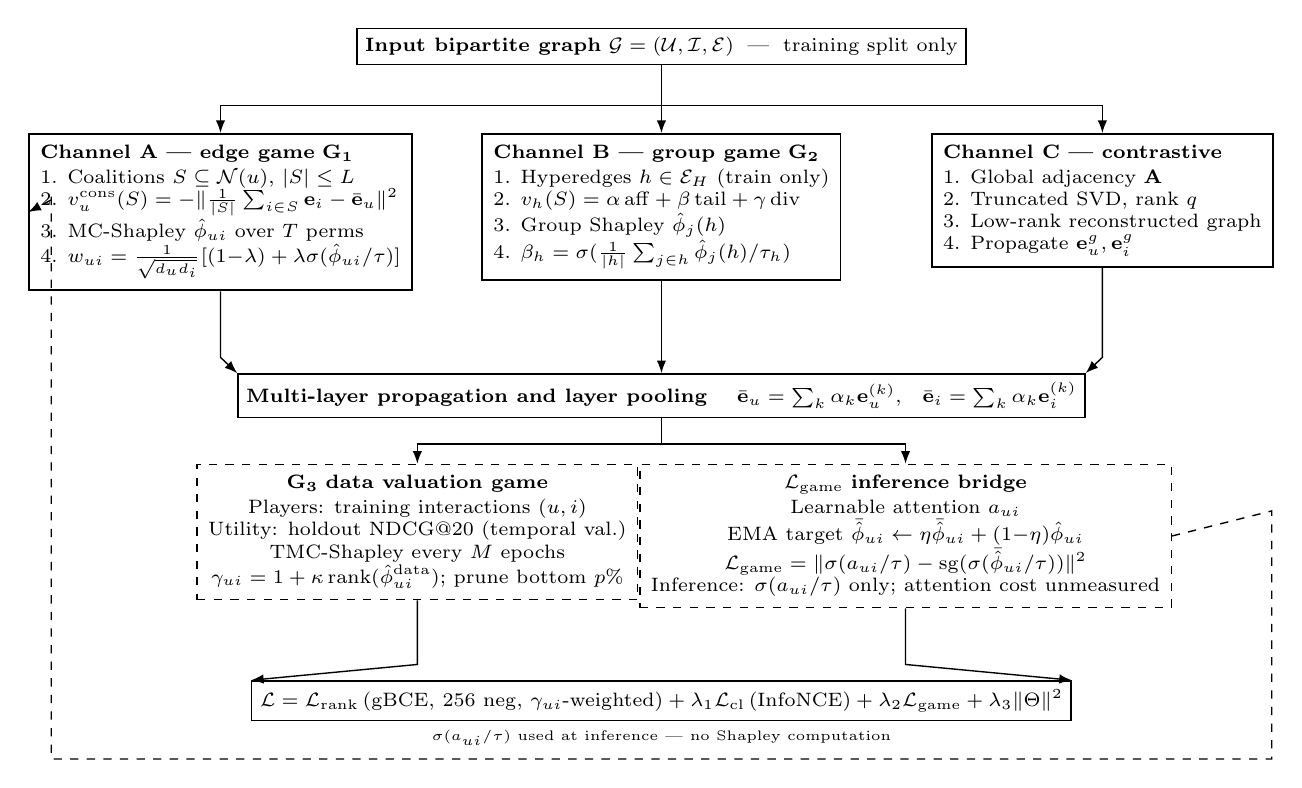
\begin{tikzpicture}
%% ---- input -----------------------------------------------------------
\node[blk, minimum width=6.2cm] (in) at (0,0)
  {\textbf{Input bipartite graph} $\mathcal{G}=(\mathcal{U},\mathcal{I},
   \mathcal{E})$ \;---\; training split only};

%% ---- three channels --------------------------------------------------
\node[chan, anchor=north] (A) at (-5.6,-1.1)
  {\textbf{Channel A --- edge game} $\mathbf{G_1}$\\[1pt]
   1. Coalitions $S\subseteq\mathcal{N}(u)$, $|S|\le L$\\
   2. $v_u^{\mathrm{cons}}(S)=-\lVert\frac{1}{|S|}\sum_{i\in S}
      \mathbf{e}_i-\bar{\mathbf{e}}_u\rVert^2$\\
   3. MC-Shapley $\hat{\phi}_{ui}$ over $T$ perms\\
   4. $w_{ui}=\frac{1}{\sqrt{d_ud_i}}[(1{-}\lambda)+\lambda
      \sigma(\hat{\phi}_{ui}/\tau)]$};

\node[chan, anchor=north] (B) at (0,-1.1)
  {\textbf{Channel B --- group game} $\mathbf{G_2}$\\[1pt]
   1. Hyperedges $h\in\mathcal{E}_H$ (train only)\\
   2. $v_h(S)=\alpha\,\mathrm{aff}+\beta\,\mathrm{tail}
      +\gamma\,\mathrm{div}$\\
   3. Group Shapley $\hat{\phi}_j(h)$\\
   4. $\beta_h=\sigma(\frac{1}{|h|}\sum_{j\in h}
      \hat{\phi}_j(h)/\tau_h)$};

\node[chan, anchor=north] (C) at (5.6,-1.1)
  {\textbf{Channel C --- contrastive}\\[1pt]
   1. Global adjacency $\mathbf{A}$\\
   2. Truncated SVD, rank $q$\\
   3. Low-rank reconstructed graph\\
   4. Propagate $\mathbf{e}^g_u,\mathbf{e}^g_i$};

%% ---- pooling ---------------------------------------------------------
\node[blk, minimum width=9.4cm, anchor=north] (pool) at (0,-4.15)
  {\textbf{Multi-layer propagation and layer pooling} \quad
   $\bar{\mathbf{e}}_u=\sum_k\alpha_k\mathbf{e}^{(k)}_u$, \;
   $\bar{\mathbf{e}}_i=\sum_k\alpha_k\mathbf{e}^{(k)}_i$};

%% ---- G3 and the bridge ----------------------------------------------
\node[band, anchor=north, minimum width=4.6cm] (G3) at (-3.1,-5.3)
  {$\mathbf{G_3}$ \textbf{data valuation game}\\[1pt]
   Players: training interactions $(u,i)$\\
   Utility: holdout NDCG@20 (temporal val.)\\
   TMC-Shapley every $M$ epochs\\
   $\gamma_{ui}=1+\kappa\,\mathrm{rank}(\hat{\phi}^{\mathrm{data}}_{ui})$;
   prune bottom $p\%$};

\node[band, anchor=north, minimum width=4.6cm] (LG) at (3.1,-5.3)
  {$\mathcal{L}_{\mathrm{game}}$ \textbf{inference bridge}\\[1pt]
   Learnable attention $a_{ui}$\\
   EMA target $\bar{\hat{\phi}}_{ui}\leftarrow
   \eta\bar{\hat{\phi}}_{ui}+(1{-}\eta)\hat{\phi}_{ui}$\\
   $\mathcal{L}_{\mathrm{game}}=
   \lVert\sigma(a_{ui}/\tau)-\mathrm{sg}(\sigma(\bar{\hat{\phi}}_{ui}/\tau))\rVert^2$\\
   Inference: $\sigma(a_{ui}/\tau)$ only; attention cost unmeasured};

%% ---- objective -------------------------------------------------------
\node[blk, minimum width=9.4cm, anchor=north] (loss) at (0,-8.05)
  {$\mathcal{L}=\mathcal{L}_{\mathrm{rank}}\,(\text{gBCE},\,256\ \text{neg},\,
   \gamma_{ui}\text{-weighted})
   +\lambda_1\mathcal{L}_{\mathrm{cl}}\,(\text{InfoNCE})
   +\lambda_2\mathcal{L}_{\mathrm{game}}+\lambda_3\lVert\Theta\rVert^2$};

%% ---- arrows ----------------------------------------------------------
\draw[ar] (in.south) -- (0,-0.75) -- (-5.6,-0.75) -- (A.north);
\draw[ar] (in.south) -- (B.north);
\draw[ar] (in.south) -- (0,-0.75) -- (5.6,-0.75) -- (C.north);

\draw[ar] (A.south) -- (-5.6,-3.95) -- (pool.north west);
\draw[ar] (B.south) -- (pool.north);
\draw[ar] (C.south) -- (5.6,-3.95) -- (pool.north east);

\draw[ar] (pool.south) -- (0,-5.05) -- (-3.1,-5.05) -- (G3.north);
\draw[ar] (pool.south) -- (0,-5.05) -- (3.1,-5.05) -- (LG.north);

\draw[ar] (G3.south) -- (-3.1,-7.85) -- (loss.north west);
\draw[ar] (LG.south)  -- (3.1,-7.85)  -- (loss.north east);

%% feedback: distilled attention returns to Channel A at inference
%% routed around the outside so it crosses no block
\draw[dashed, line width=0.5pt]
  (LG.east) -- (7.75,-5.9) -- (7.75,-9.05) -- (-7.75,-9.05) -- (-7.75,-1.9);
\draw[ar, dashed] (-7.75,-1.95) -- (A.west);
\node[font=\tiny, anchor=south] at (0,-9.0)
  {$\sigma(a_{ui}/\tau)$ used at inference --- no Shapley computation};
\end{tikzpicture}
\caption{The CoopGCN architecture. Channel~A applies edge-level Monte-Carlo
Shapley weights ($\mathbf{G_1}$) to bipartite propagation; Channel~B applies
group-level Shapley weights ($\mathbf{G_2}$) over hyperedges constructed
strictly from training interactions; Channel~C supplies a deterministic
SVD-truncated contrastive view countering dimensional collapse. The data-level
game $\mathbf{G_3}$ reweights and prunes training samples offline. The
consistency loss $\mathcal{L}_{\mathrm{game}}$ distils exponential
moving-average Shapley credit into learnable attention $a_{ui}$, which alone is
evaluated at inference (dashed path), so serving requires no game-theoretic
computation.}
\label{fig:arch}
\end{figure*}

\subsection{$\mathbf{G_1}$: the edge-level pairwise cooperative game}
\label{sec:g1}

\paragraph{Game definition}
For each user $u$ we define the local game $\Gamma_u = (\mathcal{N}(u), v_u)$
over interaction neighbours $i \in \mathcal{N}(u)$.

\paragraph{Value functions}
For every local game we define $v(\emptyset)=0$. The formulas below apply to
non-empty coalitions; we set $\mathrm{div}(S)=0$ for $|S|<2$. Embeddings used
as utility targets are stop-gradient snapshots from the current refresh, so a
coalition evaluation cannot move its own target. The default is the
\emph{consistency utility}
\begin{equation}
v_u^{\mathrm{cons}}(S) = -\Bigl\lVert \frac{1}{|S|}
\sum_{i \in S} \mathbf{e}_i - \bar{\mathbf{e}}_u \Bigr\rVert^2 ,
\label{eq:vcons}
\end{equation}
which measures how accurately coalition $S$ reconstructs $u$'s full pooled
embedding and costs $O(|S|d)$ per evaluation. Where the optimisation target is
explicitly long-tail we admit the \emph{preference-aware utility}
\begin{equation}
v_u^{\mathrm{pref}}(S) = \alpha \frac{1}{|S|} \!\sum_{i \in S}\! s_{ui}
+ \beta \,\mathrm{tail}(S) + \gamma \,\mathrm{div}(S),
\label{eq:vpref}
\end{equation}
where $\mathrm{tail}(S)$ is the proportion of $S$ in the bottom-80\%
popularity stratum and $\mathrm{div}(S) = \frac{1}{|S|(|S|-1)}\sum_{i \neq j}
(1 - \cos(\mathbf{e}_i,\mathbf{e}_j))$. The $\beta$ and $\gamma$ terms close a
specific back-door: were $v$ to reward predicted preference alone, high-degree
items would earn high credit and the game would re-encode the very bias it is
meant to remove.

\paragraph{Aggregation}
Credits enter propagation through Eq.~\eqref{eq:edgeweight}, giving
\begin{equation}
\mathbf{e}_u^{(k+1)} = \sum_{i \in \mathcal{N}(u)} w_{ui}\,
\mathbf{e}_i^{(k)} .
\end{equation}

\subsection{$\mathbf{G_2}$: the hyperedge-level group cooperative game}
\label{sec:g2}

\paragraph{Game definition}
For each hyperedge $h \in \mathcal{E}_H$---a genre combination (ML-1M),
business category (Yelp2018) or co-purchase category (Amazon-Book),
constructed strictly from the training split---we define $\Gamma_h = (h, v_h)$
whose players are the member items.

\paragraph{Value function and propagation}
We define $v_h(\emptyset)=0$, use the expression below for non-empty $S$, and
set $\mathrm{div}(S)=0$ for $|S|<2$.
\begin{equation}
v_h(S) = \alpha \frac{1}{|S|^2} \!\!\sum_{j,k \in S}\!\! \mathrm{aff}(j,k)
+ \beta\, \mathrm{tail}(S) + \gamma\, \mathrm{div}(S),
\end{equation}
with $\mathrm{aff}(j,k) = \cos(\mathbf{e}_j,\mathbf{e}_k)$ the pairwise
affinity. The group credit and hypergraph convolution are
\begin{align}
\beta_h &= \sigma \Bigl( \frac{1}{|h|} \textstyle\sum_{j \in h}
\hat{\phi}_j(h)/\tau_h \Bigr) \in (0,1), \\
\mathbf{e}_v^{(k+1)} &= \sum_{h \ni v} \frac{\beta_h}{\sqrt{D_v D_h}}
\sum_{v' \in h} \frac{1}{\sqrt{D_h}} \mathbf{e}_{v'}^{(k)} .
\end{align}
Setting $\beta_h \equiv 1$ recovers standard unweighted hypergraph CF of the
DHCN/HCCF family.

\subsection{$\mathbf{G_3}$: the data-level valuation game}
\label{sec:g3}

\paragraph{Game definition}
Players are training interactions $(u,i) \in \mathcal{B}$, with
$v^{\mathrm{ndcg}}(\emptyset)=0$ by definition; for non-empty $S$, the value
function $v^{\mathrm{ndcg}}(S)$ is holdout NDCG@20 on the temporal validation
split of a model trained on $S$.

\paragraph{Valuation, reweighting and pruning}
Full retraining per coalition being infeasible, we apply TMC-Shapley
\citep{ghorbani2019datashapley} offline every $M$ epochs to obtain
$\hat{\phi}^{\mathrm{data}}_{ui}$, then set
\begin{equation}
\gamma_{ui} = 1 + \kappa \cdot
\mathrm{rank}\bigl(\hat{\phi}^{\mathrm{data}}_{ui}\bigr) \in [1, 1+\kappa],
\end{equation}
where $\mathrm{rank}(\cdot) \in [0,1]$ is the normalised quantile rank.
Interactions in the bottom $p\%$ (we use $p = 5$) are flagged as
noise or poisoning and pruned from the training graph. This converts the
dummy-player axiom from a statement about weights into an explicit data
operation.

\subsection{Multi-task objective and consistency regularisation}
\label{sec:loss}

The end-to-end objective combines ranking, contrastive learning, game
consistency and $L_2$ regularisation:
\begin{equation}
\mathcal{L} = \mathcal{L}_{\mathrm{rank}}
+ \lambda_1 \mathcal{L}_{\mathrm{cl}}
+ \lambda_2 \mathcal{L}_{\mathrm{game}}
+ \lambda_3 \lVert \Theta \rVert^2 .
\label{eq:total}
\end{equation}

\paragraph{Ranking loss}
To mitigate head-item overconfidence (W7) we replace single-negative BPR with
generalised BCE over 256 sampled negatives, weighted by the $\mathbf{G_3}$
sample weights:
\begin{equation}
\mathcal{L}_{\mathrm{rank}} = -\frac{1}{|\mathcal{B}|}\!\!
\sum_{(u,i) \in \mathcal{B}}\!\! \gamma_{ui}
\Bigl[ \log \sigma(s_{ui}) + \!\!\sum_{j \in \mathrm{Neg}(u)}\!\!
w_j \log(1 - \sigma(s_{uj})) \Bigr],
\end{equation}
with $w_j$ the softmax weight of negative $j$ at temperature $\tau_n$.

\paragraph{Contrastive loss}
Local pooled embeddings are regularised against the Channel~C global view:
\begin{equation}
\mathcal{L}_{\mathrm{cl}} = -\sum_{u \in \mathcal{U}}
\log \frac{\exp\bigl(\mathrm{sim}(\bar{\mathbf{e}}_u,
\mathbf{e}^{g}_u)/\tau_c\bigr)}
{\sum_{u'} \exp\bigl(\mathrm{sim}(\bar{\mathbf{e}}_u,
\bar{\mathbf{e}}_{u'})/\tau_c\bigr)} .
\end{equation}

\paragraph{Shapley consistency loss}
\begin{align}
\mathcal{L}_{\mathrm{game}} &= \sum_{(u,i) \in \mathcal{E}}
\bigl\lVert \sigma(a_{ui}/\tau) -
\mathrm{sg}\!\left(\sigma(\bar{\hat{\phi}}_{ui}/\tau)\right)
\bigr\rVert^2, \label{eq:game}\\
\bar{\hat{\phi}}^{(t)}_{ui} &= \eta\, \bar{\hat{\phi}}^{(t-1)}_{ui}
+ (1-\eta)\, \hat{\phi}^{(t)}_{ui}, \quad \eta = 0.9,
\end{align}
where $a_{ui}$ is an end-to-end learnable attention weight and
$\mathrm{sg}(\cdot)$ the stop-gradient operator. The EMA buffer damps the high
variance of Monte-Carlo estimates; the stop-gradient prevents the attention
parameters from corrupting their own target.

\subsection{Inference without Monte-Carlo Shapley sampling}
\label{sec:zero}

During inference all game-theoretic computation is disabled. Because $a_{ui}$
is regularised by Eq.~\eqref{eq:game} to track $\bar{\hat{\phi}}_{ui}$,
forward propagation uses
\begin{equation}
w_{ui} = \frac{1}{\sqrt{d_u d_i}}
\bigl[(1-\lambda) + \lambda\, \sigma(a_{ui}/\tau)\bigr],
\label{eq:infweight}
\end{equation}
so no Monte-Carlo Shapley computation is performed at serving time. The
residual cost relative to LightGCN is one forward pass of the attention
network per edge, which we have not measured
(Section~\ref{sec:limitations}). The Monte-Carlo computation is paid during training and amortised into the
attention weights; this does not imply zero latency relative to LightGCN.

%==========================================================================
\section{Computational complexity and feasibility}
\label{sec:complexity}

\subsection{Restricted coalitions and permutation sampling}
\label{sec:restrict}

Exact Shapley computation via Eq.~\eqref{eq:shapley} requires
$O(2^{|\mathcal{N}|})$ evaluations. CoopGCN applies three standard
mitigations. \emph{Restricted coalitions:} for high-degree nodes,
neighbourhoods are capped at top-$L$ ($L \le 32$) by reservoir sampling.
\emph{Monte-Carlo permutation sampling:} $\hat{\phi}_{ui}$ is estimated from
$T$ random permutations per refreshed node, reducing local cost to $O(T \cdot
|\mathcal{N}| \cdot d)$. This is the polynomial sampling estimator of Castro
et al. \citep{castro2009polynomial}. It is unbiased for the restricted game
induced by the sampled, capped neighbourhood, not for the original full game;
its Monte-Carlo variance decreases as $O(1/T)$. Stratified allocation \citep{castro2017improving} would tighten the
constant further and is a straightforward extension we have not pursued here. \emph{Periodic refresh:} credits are recomputed every
$P$ epochs ($M$ for $\mathbf{G_3}$) and stored in the EMA buffer, which serves
intermediate steps. Algorithm~\ref{alg:coopgcn} gives the resulting training
loop.

\begin{algorithm}[t]
\caption{CoopGCN training}
\label{alg:coopgcn}
\small
\begin{algorithmic}[1]
\State \textbf{Input:} train graph $\mathcal{G}$, hyperedges $\mathcal{E}_H$
(train only), periods $P,M$
\State Audit split disjointness; compute $d_u,d_i$ from train edges only
\State Initialise embeddings, attention net, EMA buffer
$\bar{\hat{\phi}} \gets \mathbf{0}$
\For{epoch $t = 1 \ldots T_{\max}$}
  \If{$t \bmod P = 0$}
    \State $\hat{\phi}_{ui} \gets$ MC-Shapley on $\Gamma_u$ under
    $v^{\mathrm{cons}}$ \Comment{$\mathbf{G_1}$}
    \State $\bar{\hat{\phi}} \gets \eta \bar{\hat{\phi}} + (1-\eta)\hat{\phi}$
    \State $\hat{\phi}_j(h) \gets$ MC-Shapley on $\Gamma_h$ under $v_h$,
    $\forall h \in \mathcal{E}_H$ \Comment{$\mathbf{G_2}$}
    \State $\beta_h \gets \sigma(\mathrm{mean}_j \hat{\phi}_j(h)/\tau_h)$
  \EndIf
  \If{$t \bmod M = 0$}
    \State $\hat{\phi}^{\mathrm{data}} \gets$ TMC-Shapley under
    $v^{\mathrm{ndcg}}$ \Comment{$\mathbf{G_3}$}
    \State Set $\gamma_{ui}$; prune bottom $p\%$ from $\mathcal{G}$
    \State Recompute train degrees, tail mask and hyperedges after pruning
  \EndIf
  \For{minibatch $\mathcal{B}$}
    \State $a_{ui} \gets \mathrm{AttNet}([\mathbf{e}_u \Vert \mathbf{e}_i])$
    \State $w_{ui}$ by Eq.~\eqref{eq:edgeweight} with $\sigma(a_{ui}/\tau)$ in
    place of $\sigma(\bar{\hat{\phi}}_{ui}/\tau)$ \Comment{see Sec.~\ref{sec:gap}}
    \State Propagate Channels A, B; pool; compute $\mathbf{e}^{g}$ (Channel C)
    \State Update by Eq.~\eqref{eq:total}
  \EndFor
\EndFor
\State \textbf{Inference:} disable Shapley; use $\sigma(a_{ui}/\tau)$ only
\end{algorithmic}
\end{algorithm}

\subsection{Amortised complexity}
\label{sec:amortised}

Table~\ref{tab:complexity} summarises the analytical budget. The design
constraint is that Shapley estimation consume under 20\% of total training
time; $\mathbf{G_1}$ dominates because it is the only game defined per user
rather than per hyperedge or per batch. Serving performs no Shapley sampling, but the residual attention-network
overhead relative to LightGCN is unmeasured (Section~\ref{sec:zero}).

\begin{table}[t]
\centering
\caption{Analytical cost of each cooperative game. Percentages are design
budgets, not measured wall-clock overhead. Serving omits these estimators but
retains the attention network of Eq.~\eqref{eq:infweight}.}
\label{tab:complexity}
\footnotesize
\begin{tabular}{lllll}
\toprule
\textbf{Level} & \textbf{Estimator} & \textbf{Cost / refresh} &
\textbf{Train} & \textbf{Mem.} \\
\midrule
$\mathbf{G_1}$ & MC, $L\le32$ & $O(|\mathcal{U}| T L d)$ & $+12$--$15\%$ &
$O(|\mathcal{E}|)$ \\
$\mathbf{G_2}$ & MC, $|h|\le32$ & $O(|\mathcal{E}_H| T |h| d)$ & $+5$--$8\%$ &
$O(|\mathcal{E}_H|)$ \\
$\mathbf{G_3}$ & TMC & $O(K |\mathcal{B}_{\mathrm{val}}|)$ evals & $+4$--$6\%$ &
$O(|\mathcal{B}|)$ \\
\midrule
\textbf{Total} & Amortised & --- & Unmeasured & Unmeasured \\
\bottomrule
\end{tabular}
\end{table}

%==========================================================================
\section{Experimental design and methodology}
\label{sec:design}

\subsection{Data leakage audit and temporal evaluation protocol}
\label{sec:leakage}

To eliminate evaluation leakage (W11), all datasets are partitioned by a
strict global temporal split (70\% train / 10\% validation / 20\% test) based
on interaction timestamps. Three properties are enforced. \emph{Topological
isolation:} the adjacency matrix, node degrees $d_u,d_i$, the bottom-80\% tail
mask and all hyperedges $\mathcal{E}_H$ are computed strictly on the training
split. \emph{Verification:} an automated assertion checks
$\mathcal{E}_{\mathrm{val}} \cap \mathcal{E}_{\mathrm{train}} = \emptyset$ and
$\mathcal{E}_{\mathrm{test}} \cap \mathcal{E}_{\mathrm{train}} = \emptyset$
before training begins. \emph{Full-catalogue ranking:} evaluation ranks the
entire item catalogue at cut-off 20 with no negative sampling. We stress the
first point because computing the tail mask from full-dataset degrees---a
common shortcut---would leak test information into precisely the metric on
which we claim our largest gains.

\subsection{Benchmark datasets}
\label{sec:datasets}

The measured evidence covers five standard CF benchmarks; the three largest
span two orders of magnitude in catalogue size and roughly a factor of 70 in
density
(Table~\ref{tab:datasets}). ML-1M is the primary dense benchmark; ML-100K is a smaller dense check, and
Gowalla, Yelp2018 and Amazon-Book test generalisation to the sparse, large-catalogue regime where
credit assignment should matter most, because scarce interactions per user
leave topology-only weighting less signal to exploit.

\begin{table}[t]
\centering
\caption{Benchmark datasets and leakage-safe hyperedge construction. All
hyperedges are built from the training split only.}
\label{tab:datasets}
\footnotesize
\begin{tabular}{lrrrl}
\toprule
\textbf{Dataset} & \textbf{Users} & \textbf{Items} & \textbf{Density} &
\textbf{Hyperedges} \\
\midrule
ML-100K & 943 & 1{,}682 & 6.30\% & Genre combinations \\
ML-1M & 6{,}040 & 3{,}706 & 4.47\% & Genre combinations \\
Gowalla & 29{,}858 & 40{,}981 & 0.08\% & Geographic sessions \\
Yelp2018 & 31{,}668 & 38{,}048 & 0.13\% & Business categories \\
Amazon-Book & 52{,}643 & 91{,}599 & 0.06\% & Co-purchase categories \\
\bottomrule
\end{tabular}
\end{table}

\subsection{Baseline competitors}
\label{sec:baselines}

Nine baselines span four families: \textbf{MF}, \textbf{NCF}
\citep{he2017ncf} and \textbf{RecDCL} \citep{zhang2024recdcl} as non-graph
context; \textbf{MF} is trained with BPR \citep{rendle2009bpr}; standard graph
CF \textbf{LightGCN}
\citep{he2020lightgcn}; contrastive \textbf{SGL} \citep{wu2021sgl} and
\textbf{SimGCL} \citep{yu2022simgcl}; norm-weighted \textbf{LightGCN++}
\citep{lee2024lightgcnpp} and learned-attention \textbf{GAT-CF}; and hypergraph/cooperative \textbf{HCCF}
\citep{xia2022hccf}, \textbf{HPCF} and \textbf{DyHuCoG} \citep{louhichi2026dyhucog}.
All models use the same split and evaluator. The retained records do not
contain complete trial-by-trial search traces or a GAT-CF learning-rate sweep;
we therefore cannot verify equal tuning diligence and treat model comparisons,
especially GAT-CF collapse on sparse data, as preliminary.

\subsection{Implementation and reproducibility settings}
\label{sec:repro}

All model classes are implemented in PyTorch in the released codebase and use
the shared split and evaluator interfaces. This reduces, but cannot eliminate,
implementation drift; equivalence to each originating implementation has not
been independently established. Embeddings are $d = 64$ dimensional with $K = 3$
propagation layers, initialised $\mathcal{N}(0, 0.1^2)$. Optimisation uses
Adam at learning rate $5 \times 10^{-3}$, weight decay $\lambda_3 = 10^{-4}$,
batch size 1024 (raised to 8192 for the full-catalogue scoring pass), for at
most 1000 epochs with early stopping on validation NDCG@20 at patience 50.
The ranking loss is gBCE with 256 sampled negatives per positive.

Game-specific settings are: mixing coefficient $\lambda = 0.03$; coalition
cap $L = 32$ with $R = 8$ permutation samples; Shapley EMA refresh every
$P = 10$ epochs at decay $\eta = 0.9$; Data-Shapley curation every $M = 20$
epochs with reweighting range $\kappa$ and bottom-5\% pruning; temperatures
$\tau$ and $\tau_h$ tuned on validation only. Loss weights $\lambda_1$
(contrastive) and $\lambda_2$ (consistency) are selected per dataset on the
validation split, never on test. Evaluation scripts are in the repository named in the data-availability
statement. The retained measured record is single-run and does not preserve a
complete hardware/software manifest, seed sweep, or trial-level tuning log.

\subsection{Multi-dimensional evaluation metrics}
\label{sec:metrics}

The evaluation design defines four metric families. \emph{Ranking accuracy:}
NDCG@20 and Recall@20. \emph{Tail performance:} Tail Recall
\textbf{TR@20}, recall restricted to the bottom-80\% least-popular items.
\emph{Catalogue diversity:} \textbf{Coverage@20}, the percentage of the
catalogue appearing in any top-20 list, and the \textbf{Gini index} of
recommendation frequency. \emph{Robustness to random corruption:} degradation
under 5\%, 10\% and 20\% random noisy-edge injection. The retained common
measured record contains only NDCG@20, TR@20 and Coverage@20; we do not fill
Recall, Gini or corruption results from incompatible sources.

\subsection{Research questions}
\label{sec:rqs}

\begin{itemize}
\item[\textbf{RQ1}] \emph{Overall accuracy.} Does CoopGCN achieve competitive
NDCG@20 and Recall@20 across benchmarks of differing density?
\item[\textbf{RQ2}] \emph{Shapley versus attention.} Does Shapley-derived
weighting differ from learned attention on tail recall, coverage and
robustness?
\item[\textbf{RQ3}] \emph{Group structure and collapse.} How do Channel~B
($\mathbf{G_2}$) and Channel~C contribute to long-tail recommendation?
\item[\textbf{RQ4}] \emph{Data curation and robustness.} Does $\mathbf{G_3}$ pruning improve resilience to random edge injection?
This is an empirical question; Proposition~\ref{prop:robust} is only a
Channel-A per-edge bound.
\item[\textbf{RQ5}] \emph{Efficiency.} Does $\mathcal{L}_{\mathrm{game}}$
remove sampling from the serving path at acceptable measured cost?
\end{itemize}

\subsection{Ablation design and the central comparison}
\label{sec:central}

Table~\ref{tab:matrix} specifies the ten-configuration ablation matrix. Rows
1--5 are external reference points, rows 6--9 remove one CoopGCN component
each, and row 10 is the complete system. Configurations instantiated in the
measured full-model results are marked; row 3 is measured in the main
benchmark, while component removals are available only as projections and are
therefore not marked as empirical ablations. Rows 4 and 9 remain unmeasured.

\begin{table}[t]
\centering
\caption{Ablation matrix. \checkmark\ marks configurations reported in
Section~\ref{sec:results}; $\circ$ marks configurations specified by the
design but not instantiated in the present study.}
\label{tab:matrix}
\footnotesize
\begin{tabular}{llll}
\toprule
\textbf{\#} & \textbf{Configuration} & \textbf{Games active} & \\
\midrule
1 & LightGCN (floor) & --- & \checkmark \\
2 & LightGCN++ & --- & \checkmark \\
3 & GAT-CF (attention) & --- & \checkmark \\
4 & LightGCL & --- & $\circ$ \\
5 & DyHuCoG & $\mathbf{G_2}$ & \checkmark \\
6 & CoopGCN w/o $\mathbf{G_1}$ & $\mathbf{G_2}{+}\mathbf{G_3}$ & $\circ$ \\
7 & CoopGCN w/o $\mathbf{G_2}$ & $\mathbf{G_1}{+}\mathbf{G_3}$ & $\circ$ \\
8 & CoopGCN w/o $\mathbf{G_3}$ & $\mathbf{G_1}{+}\mathbf{G_2}$ & $\circ$ \\
9 & CoopGCN w/o $\mathcal{L}_{\mathrm{game}}$ & all & $\circ$ \\
10 & \textbf{Full CoopGCN} & all & \checkmark \\
\bottomrule
\end{tabular}
\end{table}

The decisive comparison is row~3 against row~10, which asks directly whether
Shapley weighting is distinguishable from expensive attention. We fix the
victory condition in advance: \emph{even if learnable attention matches
$\hat{\phi}$-Shapley weighting on clean-data NDCG@20, CoopGCN succeeds only if
it is superior on TR@20, Coverage@20 and noise immunity simultaneously.} Row~3 is now reported under the same split and evaluator. Clean-data TR@20
and Coverage@20 favour CoopGCN, but the noise conjunct is unmeasured and the
absence of GAT-CF tuning traces prevents a definitive causal comparison. The
central question is therefore partially, not fully, answered.

\subsection{Provenance and statistical scope}
\label{sec:provenance}

The main evidence below is the repository's retained measured record: one
executed run per model--dataset cell under the temporal split and
full-catalogue evaluator. Earlier drafts contained a separate table of
literature-derived design targets, including projected CoopGCN values of
0.2960, 0.0680 and 0.0480 NDCG@20 on ML-1M, Yelp2018 and Amazon-Book. Executed
values were 0.1994, 0.0376 and 0.0235. Because those targets are contradicted by
measurement, we remove them, their component table, their random-noise curves
and all derived figures from the results section. They remain versioned in the
repository as design-history artefacts and must not be cited as findings.

The measured record spans five datasets and ten models, matching
Table~\ref{tab:measured}. It contains NDCG@20, TR@20 and Coverage@20 but not a
complete common-protocol Recall@20 or Gini record. We do not fill missing cells
from publications with different splits. Each value is a single point
estimate: no standard deviation, confidence interval or significance test is
available, and we make no claim of statistical significance or definitive
superiority. Complete tuning traces, including a GAT-CF learning-rate sweep,
are also unavailable. The results are consequently preliminary evidence that
motivates a multi-seed confirmatory study.

%==========================================================================
\section{Results and discussion}
\label{sec:results}

\subsection{Measured evaluation across five datasets}
\label{sec:measured}

Table~\ref{tab:measured} reports the complete retained measured record. Values
are NDCG@20 / TR@20 / Coverage@20, with coverage expressed as a percentage in
every column. Bold marks the best graph model for each metric; non-graph models
are included as context because their objectives and inductive biases differ.

\begin{table*}[t]
\centering
\caption{Single-run measured NDCG@20 / TR@20 / Coverage@20 (\%). No uncertainty
intervals are available; differences must not be interpreted as statistically
significant.}
\label{tab:measured}
\scriptsize
\setlength{\tabcolsep}{2.3pt}
\begin{tabular}{lccccc}
\toprule
\textbf{Model} & \textbf{ML-100K} & \textbf{ML-1M} & \textbf{Gowalla} &
\textbf{Yelp2018} & \textbf{Amazon-Book} \\
\midrule
\textbf{CoopGCN} & 0.1826 / \textbf{0.0106} / \textbf{46.9} &
0.1994 / \textbf{0.0075} / \textbf{40.7} &
0.1089 / 0.0104 / 7.95 &
\textbf{0.0376} / \textbf{0.0006} / \textbf{5.36} &
\textbf{0.0235} / \textbf{0.0036} / \textbf{6.47} \\
LightGCN++ & 0.1627 / 0.0100 / 46.5 & 0.2054 / 0.0008 / 37.3 &
\textbf{0.1092} / \textbf{0.0116} / \textbf{8.06} &
0.0359 / \textbf{0.0006} / 5.01 & 0.0222 / 0.0027 / 5.44 \\
GAT-CF & \textbf{0.1943} / 0.0022 / 19.4 & 0.2096 / 0.0001 / 10.0 &
0.0038 / 0.0005 / 10.3 & 0.0014 / 0.0003 / 0.13 &
0.0002 / 0.0000 / 0.05 \\
LightGCN & 0.1842 / 0.0036 / 27.8 & 0.2128 / 0.0000 / 9.82 &
0.0348 / 0.0000 / 0.20 & 0.0145 / 0.0000 / 0.35 &
0.0002 / 0.0000 / 0.05 \\
HPCF & 0.1747 / 0.0020 / 25.7 & \textbf{0.2141} / 0.0000 / 9.23 &
0.0278 / 0.0000 / 0.39 & 0.0110 / 0.0000 / 0.48 &
0.0003 / 0.0000 / 0.05 \\
HCCF & 0.1723 / 0.0019 / 21.2 & 0.2070 / 0.0000 / 8.23 &
0.0291 / 0.0000 / 0.35 & 0.0113 / 0.0000 / 0.25 &
0.0002 / 0.0000 / 0.05 \\
DyHuCoG & 0.1718 / 0.0026 / 20.5 & 0.2114 / 0.0000 / 9.42 &
0.0338 / 0.0000 / 0.32 & 0.0144 / 0.0000 / 0.35 &
0.0002 / 0.0000 / 0.05 \\
\midrule
RecDCL & 0.3103 / 0.0000 / 13.1 & 0.2997 / 0.0000 / 5.42 &
0.0434 / 0.0000 / 0.27 & 0.0109 / 0.0000 / 0.25 &
0.0042 / 0.0000 / 0.05 \\
NCF & 0.2939 / 0.0000 / 6.54 & 0.2883 / 0.0000 / 4.80 &
0.0444 / 0.0000 / 0.79 & 0.0129 / 0.0000 / 0.84 &
0.0062 / 0.0001 / 0.54 \\
MF & 0.1467 / 0.0052 / 34.5 & 0.2043 / 0.0003 / 17.1 &
0.0004 / 0.0006 / 6.70 & 0.0006 / 0.0006 / 6.82 &
0.0003 / 0.0000 / 0.05 \\
\bottomrule
\end{tabular}
\end{table*}

\subsection{RQ1: accuracy is regime-dependent}
\label{sec:rq1}

Within the direct hypergraph/cooperative peer group (HCCF, HPCF and DyHuCoG),
CoopGCN has the highest point-estimate NDCG@20 on four of five datasets. It is
not uniformly superior. On ML-1M its 0.1994 is below HPCF (0.2141), LightGCN
(0.2128), DyHuCoG (0.2114), GAT-CF (0.2096), HCCF (0.2070) and LightGCN++
(0.2054). On Gowalla it is effectively tied with LightGCN++ (0.1089 versus
0.1092). On Yelp2018 and Amazon-Book it has the highest graph-model point
estimate (0.0376 and 0.0235), only 4.7\% and 5.9\% above LightGCN++.
Single-run evidence cannot establish that these small margins survive seed or
tuning variation.

The non-graph context changes the dense-data interpretation. RecDCL reaches
0.3103 and 0.2997 on ML-100K and ML-1M, respectively, while NCF reaches 0.2939
and 0.2883---roughly 35--60\% above the best graph-model point estimates. Both
methods have zero TR@20 on these datasets and markedly lower coverage, so they
occupy a head-accuracy extreme rather than uniformly dominating the measured
outcomes. Nevertheless, their scale shows that graph-based credit assignment
is not the strongest lever for dense-benchmark NDCG in this record. CoopGCN's
case must therefore rest on a different accuracy--exposure operating point and
on sparse-regime behavior, not on a general claim that graph propagation is the
best dense-data architecture.

The retained ML-1M log has contrastive loss around 5.0 against ranking loss
around 0.11, consistent with over-regularisation, but this post-hoc observation
does not prove causation. A per-dataset $\lambda_1$ sweep and measured
component ablation are needed.

\subsection{RQ2: long-tail exposure and learned attention}
\label{sec:rq2}

The distributional point estimates are larger and consistent within the direct
peer group. CoopGCN has the highest TR@20 and Coverage@20 among HCCF, HPCF and
DyHuCoG on all five datasets. On ML-1M it reaches TR@20 $=0.0075$ and coverage
$=40.7\%$, while those three peers have TR@20 $=0$ and coverage between 8.23\%
and 9.42\%. On Amazon-Book, its coverage is 6.47\% versus 0.05\% for each
peer. LightGCN++ remains a strong comparator and slightly exceeds CoopGCN on
both TR@20 and coverage on Gowalla.

GAT-CF is stronger in NDCG on ML-100K and ML-1M, but its NDCG falls to 0.0038,
0.0014 and 0.0002 on Gowalla, Yelp2018 and Amazon-Book. This could reflect a
real sparse-regime limitation or an implementation/tuning failure: learned
attention has greater capacity than fixed LightGCN weighting, and its roughly
tenfold deficit to LightGCN on Yelp2018 is anomalous. Because the retained
artefacts contain neither learning-rate sweeps nor training curves, we cannot
rule out the latter. The fair conclusion is that the measured configuration
of GAT-CF collapsed, not that attention generally fails. The same standard
applies to MF: its NDCG@20 falls to 0.0004 on Gowalla and 0.0003 on
Amazon-Book, far below its dense-data values, without retained tuning traces
that distinguish a genuine sparse-regime failure from an implementation or
optimisation artifact. Neither collapse supports an architecture-wide claim.
The pre-specified three-part victory condition is only partly met: CoopGCN
leads the retained GAT-CF configuration on tail recall and coverage, while
measured comparative noise resilience is absent.

\subsection{Descriptive accuracy--coverage sensitivity}
\label{sec:tradeoff}

A weaker ranker could mechanically expose more items, so coverage gains alone
do not identify a credit-assignment effect. As a descriptive sensitivity
check, Table~\ref{tab:tradeoff} reports Spearman rank correlation between
NDCG@20 and Coverage@20 across the ten model point estimates and, separately,
across the seven graph models. The calculation is regenerated from
\texttt{data/measured\_results.csv} by
\texttt{scripts/analyze\_measured\_tradeoff.py}.

\begin{table}[t]
\centering
\caption{Descriptive Spearman $\rho$ between NDCG@20 and Coverage@20 across
single-run model point estimates. This is a sensitivity diagnostic, not a
seed-level test or causal estimate.}
\label{tab:tradeoff}
\footnotesize
\begin{tabular}{lrr}
\toprule
\textbf{Dataset} & \textbf{All models ($n=10$)} &
\textbf{Graph models ($n=7$)} \\
\midrule
ML-100K & $-0.636$ & $-0.179$ \\
ML-1M & $-0.842$ & $-0.607$ \\
Gowalla & $0.006$ & $-0.107$ \\
Yelp2018 & $0.305$ & $0.775$ \\
Amazon-Book & $0.841$ & $0.885$ \\
\bottomrule
\end{tabular}
\end{table}

The signs are not uniformly negative: the dense benchmarks show an
accuracy--coverage trade-off, Gowalla is near zero, and the two largest sparse
catalogues show positive association. This rules out a universal mechanical
explanation in which lower NDCG necessarily produces higher coverage, but it
does not isolate CoopGCN's mechanism. The sample is only 7--10 heterogeneous
models per dataset, contains ties, and inherits all single-run and tuning
limitations of Table~\ref{tab:measured}; measured component ablations remain
necessary for causal attribution.

\subsection{RQ3--RQ4: component attribution and random-noise resilience remain open}
\label{sec:rq34}

The earlier component and random-edge-injection tables used projected full
model values, including ML-1M NDCG@20 $=0.2960$, that conflict with the
measured 0.1994. They cannot support claims that $\mathbf{G_1}$ accounts for
62.2\% of tail recall or that CoopGCN loses only 5.4\% under 20\% injection.
We therefore remove those tables and answer neither RQ3 nor RQ4 empirically.
Required confirmatory experiments are measured leave-one-component-out runs,
including $w/o\ \mathcal{L}_{\mathrm{game}}$, and independently retrained
0/5/10/20\% random-injection curves for CoopGCN, GAT-CF, LightGCN++ and
LightGCN. Proposition~\ref{prop:robust} remains a local Channel-A statement and
must not be read as a substitute for these experiments.

\subsection{RQ5: serving-path computation is reduced, not timed}
\label{sec:rq5}

Equation~\eqref{eq:infweight} removes Monte-Carlo Shapley estimation from the
serving path by construction. It does not make inference identical to
LightGCN: the learned attention network still executes once per edge. No
wall-clock latency, training-time overhead, peak memory or distillation-gap
measurement is retained. RQ5 therefore remains open.

\subsection{Discussion}
\label{sec:discussion}

The measured evidence suggests an accuracy--exposure frontier rather than
uniform dominance. CoopGCN changes which items are exposed, and the effect is
largest against direct hypergraph/cooperative peers in sparse catalogues. On
dense ML-1M, that redistribution coincides with lower NDCG. Because every cell
is a single run and baseline tuning traces are incomplete, even this
regime-dependent interpretation is a hypothesis supported by preliminary
point estimates, not a statistically established result. Accordingly, this
manuscript should be read as a methods paper with Stage-1-style preliminary
validation: the architecture, local theory, leakage controls and falsification
criteria are complete, whereas confirmatory component, noise, timing,
attribution and multi-seed studies are not.

%==========================================================================
\section{Conclusion, limitations and future work}
\label{sec:conclusion}

\subsection{Conclusion}

CoopGCN proposes a tri-level, Shapley-derived credit-assignment framework for
graph collaborative filtering. The exact credits satisfy the Shapley axioms;
the deployed sigmoid- and attention-based weights do not. They retain only a
credit-ordering signal within a fixed degree context, subject to Monte-Carlo
and distillation error. Channel~A exactly recovers LightGCN propagation at
$\lambda=0$ when the other channels are disabled, and
Proposition~\ref{prop:robust} bounds only a single edge's Channel-A deviation
from its zero-credit reference.

Single-run measurements suggest that CoopGCN substantially broadens tail and
catalogue exposure relative to direct hypergraph/cooperative peers and remains
competitive on sparse datasets. They also show a clear failure on dense ML-1M,
where CoopGCN has the lowest NDCG among the measured graph models. The data do
not establish universal accuracy, robustness, explainability or efficiency
superiority. The contribution at this stage is a coherent architecture,
carefully delimited theory, and preliminary evidence for an
accuracy--exposure trade-off that now requires confirmatory evaluation.

\subsection{Limitations}
\label{sec:limitations}

\textbf{Single-run evidence.} No seed variance, confidence interval or
significance test is available. Small sparse-data margins over LightGCN++ and
the sign of the dense-data deficit require at least five independent runs or
user-level bootstrap intervals before comparative claims are warranted.

\textbf{Projection artefacts are not evidence.} Earlier projected accuracy,
component and random-noise tables are contradicted by measurement and have
been removed from the results section. Consequently RQ3 and RQ4 remain open.

\textbf{Baseline tuning cannot be audited completely.} Shared splits and the
evaluator are available, but trial-level logs and GAT-CF training curves are
not. The sparse GAT-CF collapse may be a tuning or implementation artefact.

\textbf{Theory is local.} Proposition~\ref{prop:robust} is a per-edge,
per-layer Channel-A bound relative to a non-zero reference. It neither bounds
multi-layer/full-model perturbation nor NDCG degradation. The full weight
retains degree normalisation, and efficiency and additivity apply to $\phi$,
not deployed weights.

\textbf{Attribution is not validated.} Credits are structurally available,
but no deletion, insertion, stability or explainer-comparison experiment has
been executed. They must not be described as faithful explanations.

\textbf{Efficiency is not measured.} Serving omits Shapley sampling but retains
an attention network. Training time, inference latency, memory and the
worst-case distillation gap $\delta$ are unknown.

\textbf{Scope and validation reuse.} Hyperedges depend on metadata; all
metrics are reported at one cut-off; random corruption and targeted poisoning
have not been measured in the retained evidence; and complete preprocessing
manifests and hyperparameter-search traces are unavailable. Repeated
$\mathbf{G_3}$ valuation on the same validation split may overfit that holdout;
a nested valuation split is required in confirmatory work.

\subsection{Future work}
\label{sec:future}

The immediate confirmatory study should (i) run at least five seeds with a
fixed and published search budget; (ii) retain training curves and selected
hyperparameters for GAT-CF and every comparator; (iii) execute measured
component, $w/o\ \mathcal{L}_{\mathrm{game}}$ and random-injection ablations;
(iv) report wall-clock and memory measurements; and (v) execute the attribution
protocol below. Until those experiments are complete, extending the model to
targeted attacks, metadata-free graphs, sequential recommendation or streaming
graphs is secondary.

\subsection{A pre-specified protocol for evaluating the attributions}
\label{sec:xai-protocol}

Because the explainability claim is the one most likely to be over-read, we
fix in advance what would falsify it. Four tests, in increasing order of
stringency.

\emph{Deletion (necessity).} Remove the top-$k$ interactions of user $u$ by
$\hat{\phi}_{ui}$, re-score without retraining, and record the drop in
$s_{ui}$ for the target item. Compare against removing $k$ random
interactions and $k$ highest-degree interactions. A faithful attribution must
produce a steeper degradation curve than both.

\emph{Insertion (sufficiency).} Starting from the empty history, re-introduce
interactions in descending $\hat{\phi}_{ui}$ order and record how quickly
$s_{ui}$ recovers. Report the area under both curves, the standard
comprehensiveness and sufficiency summary.

\emph{Stability.} Recompute $\hat{\phi}_{ui}$ across seeds and across $R \in
\{4, 8, 16, 32\}$ permutations, and report rank correlation between runs.
Monte-Carlo attribution with $R = 8$ may not be rank-stable; if it is not, the
attributions are unusable as explanations even if the recommender itself
performs well.

\emph{Comparison.} Repeat all three against GNNExplainer
\citep{ying2019gnnexplainer}, PGExplainer \citep{luo2020pgexplainer} and
SubgraphX \citep{yuan2021subgraphx}, the last being the closest competitor
since it also uses Shapley values on graphs.

The victory condition is that $\hat{\phi}$ dominates degree and random
baselines on deletion and insertion \emph{and} attains rank correlation above
$0.8$ across seeds. Until these are run, the explainability contribution of
this work is a design property, not a result.

%==========================================================================
\printcredits

\section*{Declaration of competing interest}

The authors declare that they have no known competing financial interests or
personal relationships that could have appeared to influence the work reported
in this paper.

\section*{Ethics and research integrity}

This study uses five publicly released recommendation benchmarks
(MovieLens-100K, MovieLens-1M, Gowalla, Yelp2018 and Amazon-Book) and recruits
no human participants. The main table reports single-run measured records; it
does not report uncertainty or statistical significance. Projection-only
leaderboards, ablations and random-noise curves from earlier drafts are not
presented as findings. The measured Shapley-versus-attention comparison is
partial: clean-data metrics are available, comparative noise resilience and a
complete GAT-CF tuning audit are not. Per-interaction credits are potentially
sensitive behavioural artefacts and, absent the pre-specified faithfulness
tests, are not represented as validated explanations.

\section*{Declaration of generative AI use}

During the preparation of this work the authors used a large language model to
assist with language editing and LaTeX formatting. After using this tool, the
authors reviewed and edited the content as needed and take full responsibility
for the content of the published article.

\section*{Data availability}

The datasets analysed in this study are publicly available: MovieLens-100K
and MovieLens-1M from GroupLens, and Gowalla, Yelp2018 and Amazon-Book from
the benchmark sources documented in the repository. Source code and the retained result records are available at
\url{https://github.com/mouadlouhichi/CoopGCN}.

\bibliographystyle{cas-model2-names}
\bibliography{references}

\end{document}
